\section{The Bitcoin Network}
	\label{sec:bitcoin}

Bitcoin is a peer-to-peer electronic cash system without any trusted third party and was described by Satoshi Nakamoto in Oktober 2008\cite{nakamoto:bitcoin}. The name Bitcoin refers to both the operating network of nodes and the system's native currency. The network and protocol is usually refereed with a large B, Bitcoin, and the currency with a small b, bitcoin.\footnote{While it's convention to not capitalize currencies in the English language, it's not been widely followed in mainstream or semi-mainstream outlets. Also the plural form of currencies is equivalent to the singular. The convention will be followed in this report.}

\subsection{Digital Signatures}

Part of the solution is provided by one way asymmetric encryption utilizing the \texttt{secp256k1} elliptic curve. Asymmetric encryption or public-key encryption essentially boils down to the ability to derive a public key from a private key without the ability to derive the private key from the public key and the ability to prove ownership of a private key through signatures without disclosing the private key. Ownership of bitcoin is proved by signing a previous transaction output payable to the public key derived bitcoin address\footnote{A bitcoin address is derived from the public key by hashing the public key with both \texttt{SHA256} and \texttt{RIPEMD160}}. 

\begin{figure}[!htb]
	\hspace*{-2cm} 
	\centering
	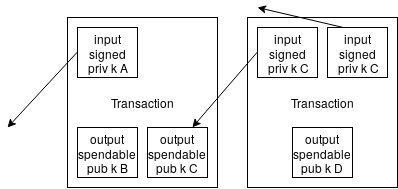
\includegraphics[width=8cm]{transaction.png}
	\caption{\textit{A simplified illustration of two transactions. 
	}}
	\label{fig:merkle:tree}
	\hspace*{2mm} 	
\end{figure}

Bitcoin is essentially a long ledger of inputs and outputs. Note that the whole output must be spent in the same transaction and usually there is an output leading back to an address the spender controls with the 'change'. The sum of all the inputs and the sum of all the outputs usually does not line up, the differential is the implicit miners fee the miner receives if the transaction is included in a block. 

\subsection{The Double-Spending problem}

While digital signatures are able prove ownership of bitcoin. There is nothing to stop the owner of an amount of bitcoin to sign multiple transactions spending the same transaction output. This is called the double-spending problem which is a variation of the more general Byzantine's General Problem.

Bitcoin solves this by using a data structure composite of a chain of blocks as seen in figure \ref{fig:blockchain}.

\begin{figure}[!htb]
	\hspace*{-2cm} 
	\centering
	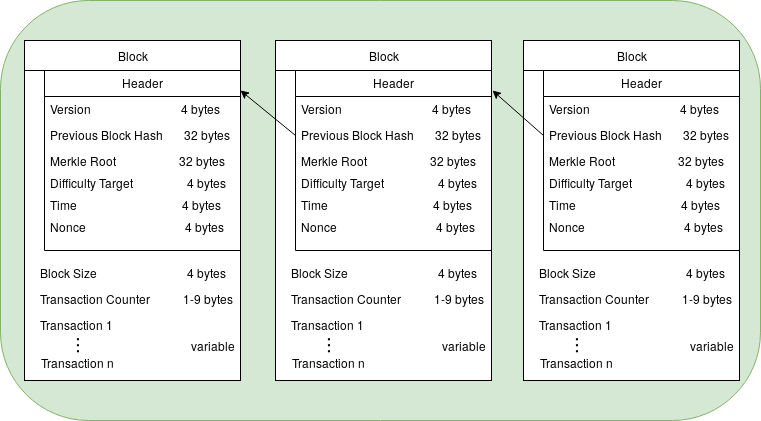
\includegraphics[width=10cm]{blockchain.png}
	\caption{\textit{The blockchain. 
	}}
	\label{fig:blockchain}
	\hspace{2mm} 
\end{figure}

The blocks are chained through the hash of the previous block's header. A block is only valid if the hash is lower than an number imposed by the difficulty target. The hash is deterministic but for all intents and purposes it is random and to find a valid hash one simply hashes the header until a valid hash is found. This process is known as \textbf{mining}. The difficulty target adjusts every 2015th\footnote{This is off by one bug, 2016 blocks is two weeks} block\cite{repository:bitcoin} and forces the average time for a block to be mined to always be ten minutes. This sort of design is known as \textit{Proof-of-Work} and bitcoin differentiate from previous implementations with the difficulty adjustment\cite{back:hashcash}\footnote{Bitcoin uses the dubble \texttt{SHA256} hash, it is essentially the same as hashcash in the cost function being non-interactive, publicly auditable, trapdoor-free and unbounded probabilistic cost\cite{back:hashcash}.}.

\subsubsection{Merkle Tree}

\begin{figure}[!htb]
	
	\centering
	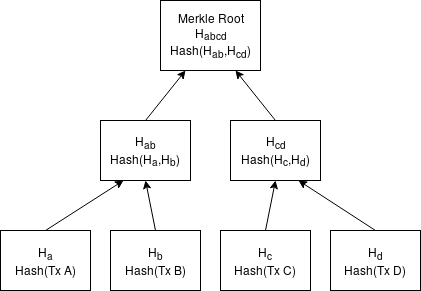
\includegraphics[width=8cm]{merkle.png}
	\caption{\textit{A merkle tree. 
	}}
	\label{fig:merkle:tree}
	
\end{figure}

The content in the block header is effectively unchangeable since a change would make the chain of hash invalid. The transactions are not in the header but are still immutable by the use of a Merkle tree(see fig \ref{fig:merkle:tree}). A Merkle tree is a tree in which the parent is the hash of its two children. The root hash of the tree is included in the header and if any transaction were to change that would cause the root hash to change rendering each transaction immutable by implication. Bitcoin uses the dubble \texttt{SHA256} as the merkle tree hash function.

\subsubsection{Incentive}

The miners are incentivized by receiving the transaction fees from the transactions included in its block as well as a subsidy. The subsidy is on the form a coinbase transacion which has only outputs, this is how new bitcoin is minted. Every fourth year the subsidy halves and by 2140 will be zero. The miner must follow the consensus rules and mined blocks not following the rules will not be propagated through the network causing the miner to loose out on the block reward. A miner controlling more than 50\% of the hashing power could technically double-spend transactions by mining blocks on an own chain without publishing them and spending on the other chain and then publish the own longer chain. A huge problem with such an attack is that the confidence of the network would decrease causing the value of the 'stolen' bitcoin to be close the worthless and still owning a lot of specialized hashing hardware worthless without the network. In a sense such an attack would cause mutual destruction for both the network and the attacker. 

\subsection{Script}

Transactions utilize a forth-like polish-notation stack based execution scripting language\cite{antonopoulos:mastering:bitcoin}. Each transaction output consist of a locking script\footnote{Also refereed to as scriptPubKey. Locking script is a broader term and technically scriptPubKey scripts $ \subseteq $ locking scripts.}. In order to spend a valid unlocking script must be provided in the input to the spending transaction that solves the locking script\footnote{scriptSig, witness $\subseteq $ unlocking scripts.}. Validation is performed by executing the unlocking script and locking script sequentially as seen in figure \ref{fig:simple:script}. 

\begin{figure}[!hbt]
	
	\begin{lstlisting}
 <@\texttt{\textcolor{red}{OP\_1}}@>   <@\texttt{\textcolor{green}{OP\_2 OP\_ADD OP\_3 OP\_EQUAL}}@>
<@\texttt{\textcolor{red}{unlock}}@>           <@\texttt{\textcolor{green}{lock}}@>
	\end{lstlisting}
	
	\caption{\textit{ A simple predicate. Evaluated from left to right (1 2 +) -> 3 and
			(3 3 =) -> true. This lock script can obviously be solved by anyone and is thus not used.
	}}
	\label{fig:simple:script}
\end{figure}

The two scripts essentially forms a predicate. If the predicate is true the transaction is true, Nakamoto considered naming the language predicate but went with script to be more inclusive to a broader audience\cite{nakamoto:predicate}.

\subsubsection{Pay to Public Key Hash}

The Pay-to-Public-key-hash or P2PKH for short was the standard script for a long time. It allows only the owner of 
the private key to the public key to spend the output.


\begin{figure}[!hbt]
	
	\begin{lstlisting}
<@\texttt{\textcolor{red}{<Sig><Pub\_Key>}}@>   
   <@\texttt{\textcolor{red}{unlock}}@>
   
<@\texttt{\textcolor{green}{OP\_DUP OP\_HASH160 <Pub\_Key\_Hash> OP\_EQUALVERIFY OP\_CHECKSIG}}@>
   <@\texttt{\textcolor{green}{lock}}@>
	\end{lstlisting}
	
	\caption{\textit{ The P2PKH locking and unlocking scripts.
	}}
	\label{fig:P2PKH}
\end{figure}

The P2PKH pushed the signature produced by the private key and the public key to the stack. The public key get duplicated and one of them get hashed. The \texttt{OP\_HASH160} is a double hash and first hashes the key with \texttt{SHA256} and then \texttt{RIPEMD160}. This is done to hide the public key until expenditure, which is useful if, for example, the ECDSA would break and private keys could be reversed. The combination of these two hashes makes it way harder to break. In the early days of the network this obfuscation technique wasn't used, for example the first transaction between Nakamoto and Finney didn't\cite{nakamoto:finney:tx}.
The \texttt{OP\_EQUALVERIFY} pops the two public key hashes and terminates the script with false if they are unequal.
The \texttt{OP\_CHECKSIG} verifies that the signature is indeed a match with the public key. 
% In the scripting language uses guard clauses than OP\_EQUALVERIFY, OP\_CHECKSIG should this be mentioned?

\subsubsection{Pay to Script Hash}

The Pay-to-Script-Hash or P2SH is a more flexible transaction than the P2PKH and was introduced with BIP016\cite{bip:0016:p2sh}. It allows the locking script to only be the hash of the redeemable script. If a cumbersome script with many public keys is considered as seen in figure \ref{fig:cumbersome:script}:

\begin{figure}
	
	\begin{lstlisting}
<@\texttt{\textcolor{red}{0 <Sig A> <Sig B>}}@>   
   <@\texttt{\textcolor{red}{unlock}}@>
	
<@\texttt{\textcolor{green}{2 <Pk\_A><Pk\_B><Pk\_C> 3 OP\_CHECKMULTISIG}}@>
   <@\texttt{\textcolor{green}{lock}}@>
	\end{lstlisting}
	
	\caption{\textit{ Showing a multisig transaction which require to signatures out of three to be spent. Note the \texttt{0} in the unlock script, it's there due to a bug with \texttt{OP\_CHECKMULTISIG} which pops an extra item from the stack. If not for the \texttt{0} it would try to pop an empty stack. The dummy value must be a \texttt{0} with BIP 147 compliant node implementations\cite{bip:0147:dummy:zero}.
	}}
	\label{fig:cumbersome:script}
\end{figure} 

This multisig transaction(in figure \ref{fig:cumbersome:script}) could be rewritten as a P2SH by hashing the locking script with \texttt{SHA256} and  \texttt{RIPEMD160} and utilizing it as seen in figure \ref{fig:p2sh}. Note that 'redeem script' refers to the lock script of figure \ref{fig:cumbersome:script} and 'redeem script hash' it's hash.

\begin{figure}[hbt!]
	
	\begin{lstlisting}
<@\texttt{\textcolor{red}{0 <Sig A> <Sig B> <redeem script> }}@>   
   <@\texttt{\textcolor{red}{unlock}}@>
	
<@\texttt{\textcolor{green}{OP\_HASH160 <redeem script hash> OP\_CHECKVERIFY}}@>
   <@\texttt{\textcolor{green}{lock}}@>
	\end{lstlisting}
	
	\caption{\textit{ The P2SH transaction which is essentially equivalent to the multisig in figure \ref{fig:cumbersome:script}
	}}
	\label{fig:p2sh}
\end{figure}

Converting to a P2SH transaction does two things:

\begin{itemize}

	\item It shifts the fee burden from the sender to the recipient. The locking script is shorter, the unlocking script is longer.
	
	\item All unspent UTXOs must be kept in the RAM of the node, shifting the burden does reduces the node RAM load. 
	
\end{itemize}

P2SH also allows the script to be used as an address(see BIP013\cite{bip:0013:p2shaddr}). By simplt sending to the script address could fund any type of complex transaction with no added complexity to the sender.

The Lightning Network utilize many complex transactions and more on this topic in section \ref{sec:lightning:network}.

\subsection{Network}

The Bitcoin network consists of nodes complying with the consensus protocol. In the beginning only the reference implementation was used but now there are multiple independent implementations\cite{repository:bitcoin}\cite{repository:btcd}\cite{repository:neutrino}.


